\documentclass{beamer}
\usepackage{pgfpages}
\setbeameroption{show notes on second screen=left} %enable for notes
\usepackage{graphicx}
\usepackage{xcolor}
\usepackage{listings}
\usepackage{hyperref}
\lstset{language=python,frame=single}
\usepackage{verbatim}
\usepackage{apacite}
\usepackage{subcaption}
\usepackage{amsmath}
\usepackage{relsize}

\usetheme[numbering=fraction]{metropolis}
%%\AtBeginSection[]
%%{
%%  \begin{frame}
%%    \frametitle{Table of Contents}
%%    \tableofcontents[currentsection]
%%  \end{frame}
%%}

%%\let\olditem\item
%%\renewcommand{\item}{\vspace{0.5\baselineskip}\olditem}
\begin{document}

\title{Learning Parallels}
\subtitle{Analogies emerge from learning dynamics in neural networks}
\author{Andrew Lampinen}
\date{3/7/2017}
\frame{\titlepage}


\section{Introduction}
\begin{frame}{Last time...}
\begin{center}
\includegraphics[width = 0.4\textwidth]{hexagon_arrow.png}
\end{center}
\end{frame}

\begin{frame}{Analogy, Transfer, and Cognition}
A variety of perspectives:
\begin{itemize}
    \item<1-> ``What makes humans smart is (1) our exceptional ability to learn by analogy'' \cite{Gentner2003} 
    \item<2-> ``Significant transfer is probably rare and accounts for very little human behavior. ... We generally do what we have learned to do and no more.'' \cite{Detterman1993}
    \item<3-> ``We found evidence for analogical transfer from a concrete, highly perceptual system to a very dissimilar domain and task ... participants' transfer was independent of their explicit reports [of awareness of the analogy between the tasks].'' \cite{Day2011}
    \item<4-> ``Our proposal is to view transfer from the perspective of preparation for future learning (PFL).'' \cite{Bransford1999} 
\end{itemize}
\note{Fortunately, there's a great deal of agreement in the field. What is the driving force? One possibility (which Bransford \& Schwartz among others acknowledged) is that there are different kinds of transfer. Failures to transfer most often occur in settings like Gick \& Holyoak's experiments with the Duncker radiation problem, where participants see one example and then have to do a symbolic mapping to another example. By contrast, successful analogical transfer often occurs in situations like Day \& Goldstone's, where participants actually interact with the system and learn about it over a period of time, or more generally in education as highlighted by Bransford \& Schwartz as the ability to learn faster in the future.}
\end{frame}

\begin{frame}{Analogy, Transfer, and Neural Networks}
If and when analogical reasoning is important for cognition, how can we solve the combinatorially explosive analogical mapping problem? Neural networks can extract analogies: 
\begin{itemize}
    \item<2-> Verbal analogies \cite{Kollias2013}
    \item<3-> Multi-task learning, zero-shot generalization \cite{Luong2016,Johnson2016}  
    \item<4-> Hinton family tree task \cite{Hinton1986}
    \begin{columns}
    \column{0.5\textwidth} Q: ``Who is Arthur's mother?'' \\ A: ``Penelope'' 
    \column{0.5\textwidth}
	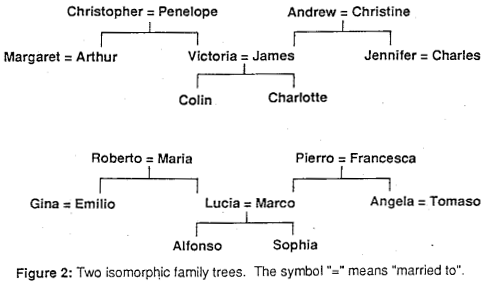
\includegraphics[width = \textwidth]{../writing/cogsci_2017/figures/hinton_family_tree_figure.png}
    \end{columns}
\end{itemize}
\uncover<5-> {Can neural networks perform amortized inference about analogies?}
\end{frame}

\section{Modeling: A toy task}
\begin{frame}{A toy task}
Learning which letters can follow other letters:\vspace{-2em}
\begin{center}
\[
\begin{array}{c|cccccc} 
& P & D & S & \pi & \delta & \sigma \\
\hline
R & 1 & 1 & 0 & 0 & 0 & 0 \\
L & 1 & 0 & 1 & 0 & 0 & 0 \\
\rho & 0 & 0 & 0 & 1 & 1 & 0\\
\lambda & 0 & 0 & 0 & 1 & 0 & 1\\
\end{array} 
\]
\end{center}
\only<2->{How, when, and why will a neural network exploit the analogy between the Latin and Greek letters?}
\end{frame}

\section{(A Little) Theory}
\begin{frame}{Linear Analyses?}
Linear neural networks:
\begin{columns}
\column{0.5\textwidth}
\begin{itemize}
    \item<2-> Learning is driven entirely by features of the SVD (Singular Value Decomposition) of the Input/Output (I/O) mapping \cite{Saxe2013}.
    \item<3-> Can we use this analysis to study analogy learning?
\end{itemize}
\column{0.5\textwidth}
    \includegraphics[width=\textwidth]{figures/linear_network_diagram.png}
\end{columns}
\note{SVD is way of factorizing a matrix into ``modes'', you can think of these kind of like components in PCA, they're ordered in terms of ``how much variance they explain.'' }
\end{frame}


\begin{frame}{Linear Analyses?}
\begin{itemize}
    \item<1-> \textbf{NO,} in the SVD of a block-diagonal matrix, the modes occur within the blocks, thus \textbf{a linear network cannot represent shared structure at convergence.}
    \uncover<2->{
    \begin{figure}
    \centering
    \begin{subfigure}{0.2\textwidth}
    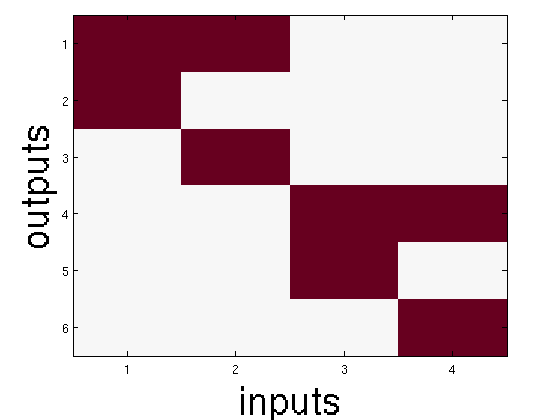
\includegraphics[width=\textwidth]{../writing/cogsci_2017/figures/nonlinear_IO.png}
    %\caption{$\Sigma_{IO}$}
    \end{subfigure}
    {\!\!\huge{$=$}\!\!}
    \begin{subfigure}{0.2\textwidth}
    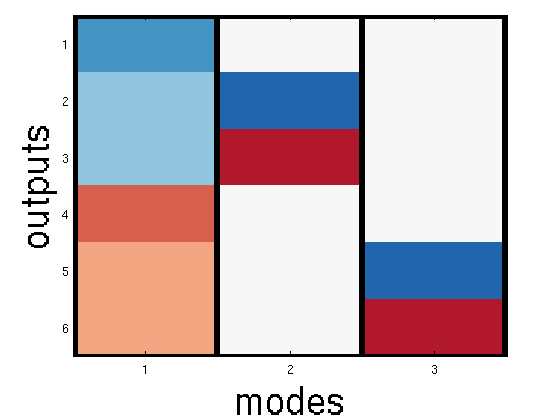
\includegraphics[width=\textwidth]{../writing/cogsci_2017/figures/U_nl.png}
    %\caption{$U$}
    \end{subfigure}
    {\!\!\LARGE{$\times$}\!\!}
    \begin{subfigure}{0.2\textwidth}
    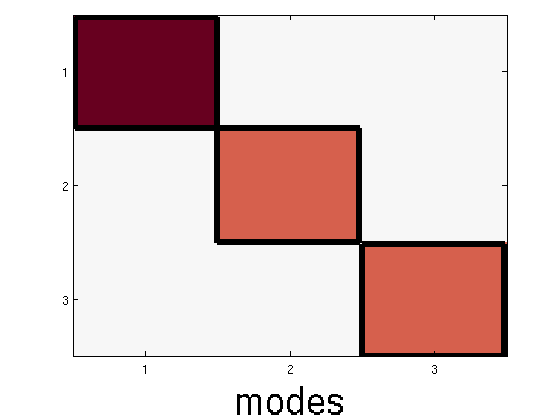
\includegraphics[width=\textwidth]{../writing/cogsci_2017/figures/S_nl.png}
    %\caption{$S$}
    \end{subfigure}
    {\!\!\LARGE{$\times$}\!\!}
    \begin{subfigure}{0.2\textwidth}
    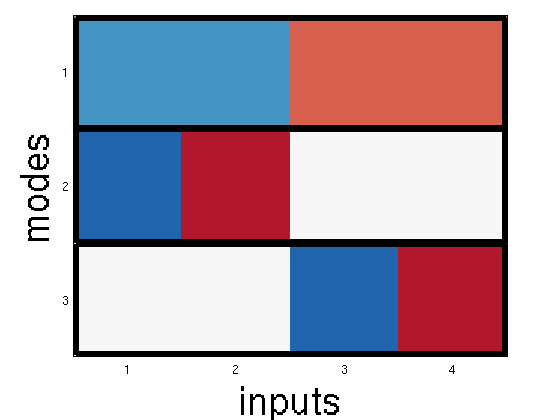
\includegraphics[width=\textwidth]{../writing/cogsci_2017/figures/V_nl.png}
    %\caption{$V^T$}
    \end{subfigure}
    \end{figure}
    }
    \item<3-> This also means that a linear network \textbf{cannot achieve as parsimonious a solution as a nonlinear network}, because it must solve each copy of a problem separately rather exploiting analogies between them.
\end{itemize}
\note{In plain english, what this means is the input output mappings for the two tasks are not really connected in any way. Really talk through SVD, first component gving strong separation between domains, and the letter that's ``always on'' in each language, second two components give within domain structure}
\end{frame}

\begin{frame}{Linearized analysis}
\begin{columns}
    \column{0.5\textwidth}
	However, we would still like to use linear analysis tools, so:
	\begin{itemize}
	    \item<2-> Train a network with a non-linearity at the output.
	    \item<3-> Perform a linearized analysis: SVD of I/O mapping of linear portion of network. 
	\end{itemize}
    \column{0.5\textwidth}
	\uncover<2->{
	\begin{center}
	    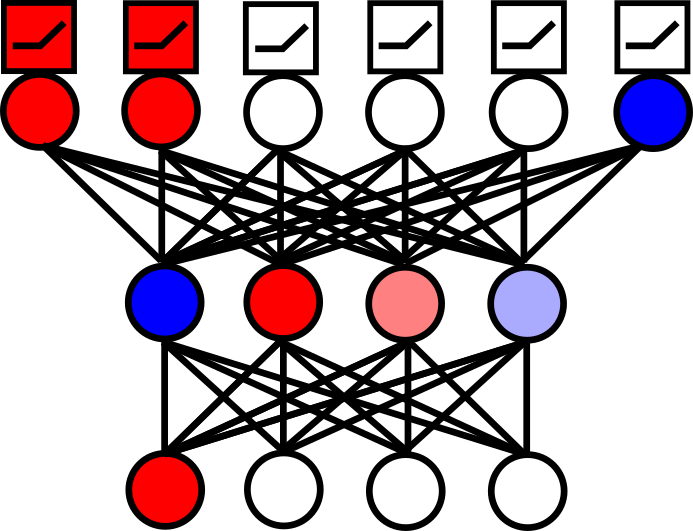
\includegraphics[width=0.8\textwidth]{../writing/cogsci_2017/figures/network_diagram.png}
	\end{center}}
\end{columns}
\note{Why use these tools? Analyzing the SVD is more principled than just looking at weights or hidden unit activations, because it is more invariant to rotations of representation space, etc.}

\end{frame}

\section{That's enough theory -- back to the task}
\begin{frame}{Toy task}
What solutions does the network discover?
\begin{columns}
    \column{0.5\textwidth}
	    \[
	    \begin{array}{c|cccccc} 
	    & P & D & S & \pi & \delta & \sigma \\
	    \hline
	    R & 1 & 1 & 0 & 0 & 0 & 0 \\
	    L & 1 & 0 & 1 & 0 & 0 & 0 \\
	    \rho & 0 & 0 & 0 & 1 & 1 & 0\\
	    \lambda & 0 & 0 & 0 & 1 & 0 & 1\\
	    \end{array} 
	    \]
    \column{0.5\textwidth}
	\begin{center}
	    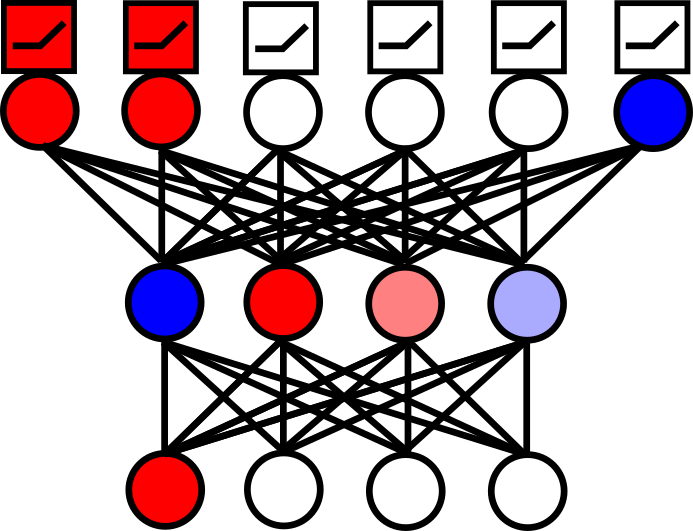
\includegraphics[width=0.8\textwidth]{../writing/cogsci_2017/figures/network_diagram.png}
	\end{center}
\end{columns}
\note{note that no weights are shared between the two tasks!}
\end{frame}

\begin{frame}{Toy task solutions}
Most commonly, the network learns an offset structure, resulting in the following linearized I/O mapping (or a symmetric analog): 
\[
\left[ \begin{matrix} 
1 & 1 & 0 & 0 & 0 & -1 \\
1 & 0 & 1 & 0 & -1 & 0 \\
 0 & 0 & -1 & 1 & 1 & 0\\
 0 & -1 & 0 & 1 & 0 & 1\\
\end{matrix}  \right] 
\]
\only<2->{(This is certainly not the only solution that can occur, but this happens about 75\% of the time. The remaining 25\% no analogy is discovered.)}
\end{frame}

\begin{frame}{Comparing SVDs}
\begin{itemize}
    \item<1-> Non-linear I/O Mapping
    \uncover<1->{
    \begin{figure}
    \centering
    \begin{subfigure}{0.2\textwidth}
    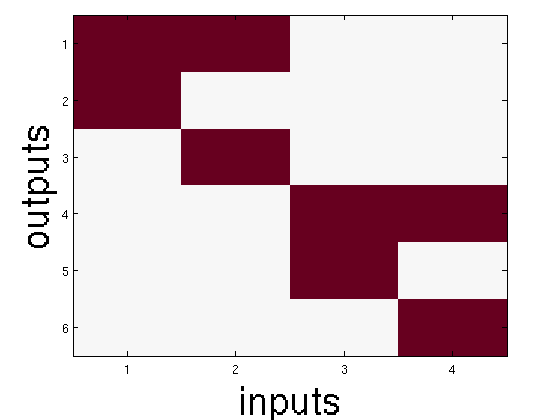
\includegraphics[width=\textwidth]{../writing/cogsci_2017/figures/nonlinear_IO.png}
    \caption{$\Sigma_{IO}$}
    \end{subfigure}
    \raisebox{0.5em}{\!\!\huge{$=$}\!\!}
    \begin{subfigure}{0.2\textwidth}
    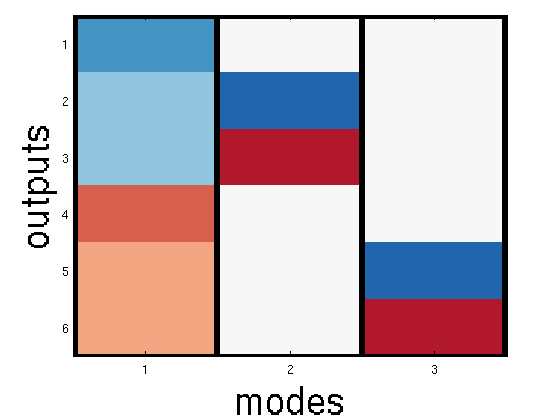
\includegraphics[width=\textwidth]{../writing/cogsci_2017/figures/U_nl.png}
    \caption{$U$}
    \end{subfigure}
    \raisebox{0.5em}{\!\!\LARGE{$\times$}\!\!}
    \begin{subfigure}{0.2\textwidth}
    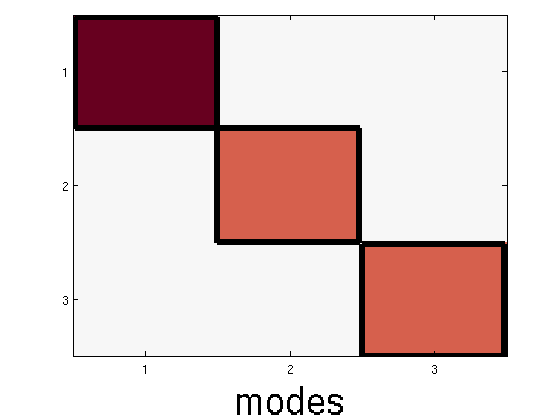
\includegraphics[width=\textwidth]{../writing/cogsci_2017/figures/S_nl.png}
    \caption{$S$}
    \end{subfigure}
    \raisebox{0.5em}{\!\!\LARGE{$\times$}\!\!}
    \begin{subfigure}{0.2\textwidth}
    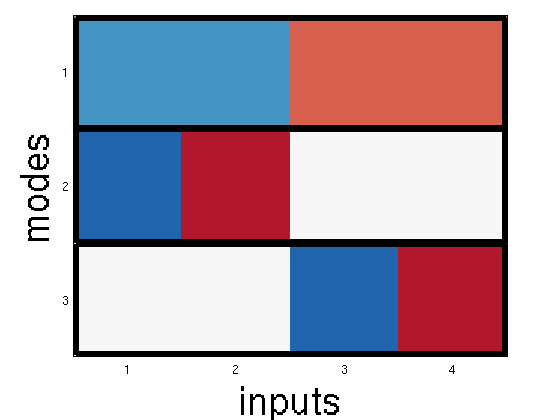
\includegraphics[width=\textwidth]{../writing/cogsci_2017/figures/V_nl.png}
    \caption{$V^T$}
    \end{subfigure}
    \end{figure}
    }
    \item<2-> Linearized I/O Mapping
    \uncover<2->{
    \begin{figure}
    \centering
    \begin{subfigure}{0.2\textwidth}
    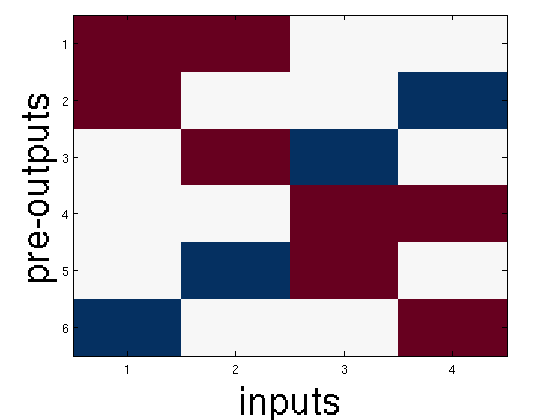
\includegraphics[width=\textwidth]{../writing/cogsci_2017/figures/linearized_IO.png}
    \caption{$\Sigma_{IO}$}
    \end{subfigure}
    \raisebox{0.5em}{\!\!\huge{$=$}\!\!}
    \begin{subfigure}{0.2\textwidth}
    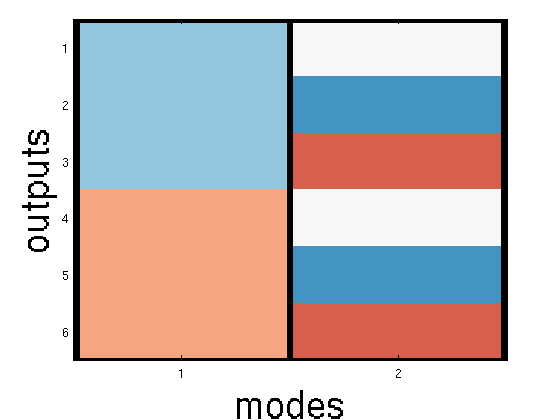
\includegraphics[width=\textwidth]{../writing/cogsci_2017/figures/U_lz.png}
    \caption{$U$}
    \end{subfigure}
    \raisebox{0.5em}{\!\!\LARGE{$\times$}\!\!}
    \begin{subfigure}{0.2\textwidth}
    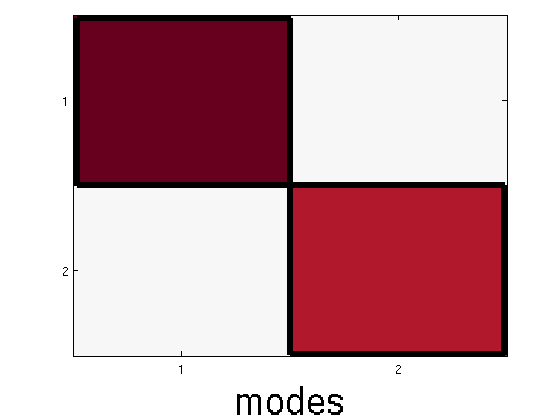
\includegraphics[width=\textwidth]{../writing/cogsci_2017/figures/S_lz.png}
    \caption{$S$}
    \end{subfigure}
    \raisebox{0.5em}{\!\!\LARGE{$\times$}\!\!}
    \begin{subfigure}{0.2\textwidth}
    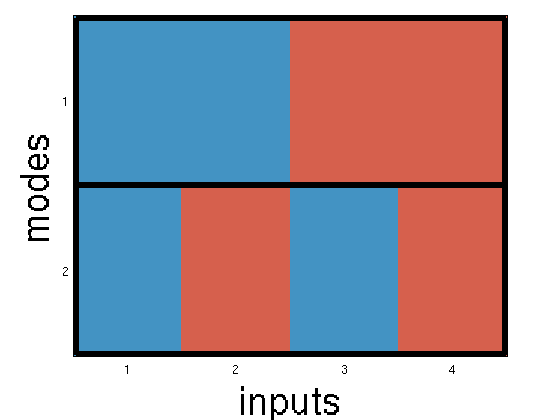
\includegraphics[width=\textwidth]{../writing/cogsci_2017/figures/V_lz.png}
    \caption{$V^T$}
    \end{subfigure}
    \end{figure}
    }
    \item<3-> Linearized I/O shows network has captured the shared structure!
\end{itemize}
\note{Can interpret the top SVD in several ways, as the task that a linear network solves, or as the task that a non-linear netwokr begins solving when it is still in the linear regime. Note more parsimonious solutions available with linearized mapping -- i.e. lower rank.}
\end{frame}

\begin{frame}{Learning dynamics}
But why and how does this occur? The linearized SVD cannot tell us, but the progression is fairly consistent: \\[11pt]
\begin{columns}
    \column{0.45\textwidth}
    \uncover<2->{Initial:{\relsize{-1}
    \[ 
    \left[ \begin{matrix} 
    0 & 0 & 0 & 0 & 0 & 0 \\
    \vdots & \vdots &\vdots &\vdots &\vdots &\vdots \\
     0 & 0 & 0 & 0 & 0 & 0\\
    \end{matrix}  \right] 
    \] 
    }}
    \uncover<4->{Base rates by domain:{\relsize{-1}
    \[
    \left[ \begin{matrix} 
    1 & 0.5 & 0.5 & 0 & 0 & 0 \\
    1 & 0.5 & 0.5 & 0 & 0 & 0 \\
    0 & 0 & 0 & 1 & 0.5 & 0.5  \\
    0 & 0 & 0 & 1 & 0.5 & 0.5  \\
    \end{matrix}  \right] 
    \]
    }
    }
    \column{0.45\textwidth}
    \uncover<3->{Base rates:{\relsize{-1}
    \[ 
    \left[ \begin{matrix} 
    0.5 & 0.25 & 0.25 & 0.5 & 0.25 & 0.25 \\
    \vdots & \vdots &\vdots &\vdots &\vdots &\vdots \\
     0.5 & 0.25 & 0.25 & 0.5 & 0.25 & 0.25\\
    \end{matrix}  \right] 
    \] 
    }}
    \uncover<5->{Solution with offsets:{\relsize{-1}
    \[
    \left[ \begin{matrix} 
    1 & 1 & 0 & 0 & 0 & -1 \\
    1 & 0 & 1 & 0 & -1 & 0 \\
     0 & 0 & -1 & 1 & 1 & 0\\
     0 & -1 & 0 & 1 & 0 & 1\\
    \end{matrix}  \right] 
    \]
    }}
\end{columns}
\uncover<6->{For all but the last step, linear network learning dynamics are very similar! Do linear networks also start to extract some shared structure?}
\note{base rates by domain = first component of SVD}
\end{frame}

\begin{frame}{Learning dynamics}
In fact, linear networks begin to extract the analogy as well, but must discard it to achieve their optimal solution.
\begin{center}
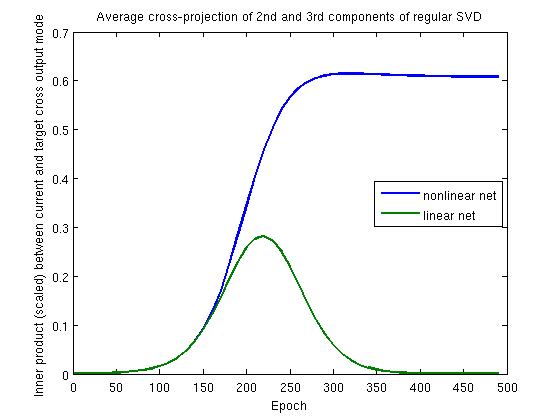
\includegraphics[width=0.7\textwidth]{../writing/cogsci_2017/figures/SVD_cross_projection_learning.png}
\end{center}
\end{frame}

\begin{frame}{Learning dynamics}
Why? When gradually learning analogous tasks simultaneously, extracting the analogy reduces error. \\[11pt]
\begin{columns}
    \column{0.45\textwidth}
    \only<1->{Base rates by domain:{\relsize{-1}
    \[
    \left[ \begin{matrix} 
    1 & 0.5 & 0.5 & 0 & 0 & 0 \\
    1 & 0.5 & 0.5 & 0 & 0 & 0 \\
    0 & 0 & 0 & 1 & 0.5 & 0.5  \\
    0 & 0 & 0 & 1 & 0.5 & 0.5  \\
    \end{matrix}  \right] 
    \]
    }
    }
    \column{0.45\textwidth}
    \only<2->{Base rates + a little shared structure{ \relsize{-1}
    \[
    \left[ \begin{matrix} 
    1 & 0.6 & 0.4 & 0 & 0.1 & -0.1 \\
    1 & 0.4 & 0.6 & 0 & -0.1 & 0.1 \\
    0 & 0.1 & -0.1 & 1 & 0.6 & 0.4  \\
    0 & -0.1 & 0.1 & 1 & 0.4 & 0.6  \\
    \end{matrix}  \right] 
    \] 
    }}
\end{columns}
\uncover<3->{More explicitly: 
{ \relsize{-1}
\[
\begin{array}{cccccc||c||cccccc} 
\multicolumn{6}{c||}{\text{output error}}  & \text{unit}  & \multicolumn{6}{c}{\text{unit output weight updates}} \\
\hline
 0 & + & - & 0 & 0 & 0  &   +    &  0 & + & - & 0 & 0 & 0   \\
0 & - & + & 0 & 0 & 0  &   -  & 0 & + & - & 0 & 0 & 0   \\
 0 & 0 & 0 & 0 & + & - &   +   &  0 & 0 & 0 & 0 & + & - \\
 0 & 0 & 0 & 0 & - & +  &  - &  0 & 0 & 0 & 0 & + & - \\
\hline
\multicolumn{7}{r}{\text{net output weight update:}} &   0 & + & - & 0 & + & - \\
\end{array} 
\]
}
} 
\note{So network will exploit the analogy to reduce error, even though no weights are shared, and even if it must discard it in the linear case.}
\end{frame}

\begin{frame}{Interim Summary}
 In this simple task:
\begin{itemize}
    \item<2-> Representation of the analogy emerges naturally from the learning dynamics (75\% of the time).
    \item<3-> This does not depend on shared weights, gradually learning two analogous tasks simultaneously suffices.
\end{itemize}
\end{frame}

\section{A more interesting example: Hinton's family tree task}
\begin{frame}{Hinton family tree task}
\begin{columns}
    \column{0.5\textwidth}
    \begin{center}
	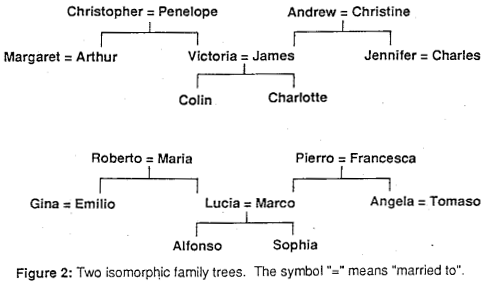
\includegraphics[width = \textwidth]{../writing/cogsci_2017/figures/hinton_family_tree_figure.png}
    \end{center}
    \column{0.5\textwidth}
    \begin{center}
	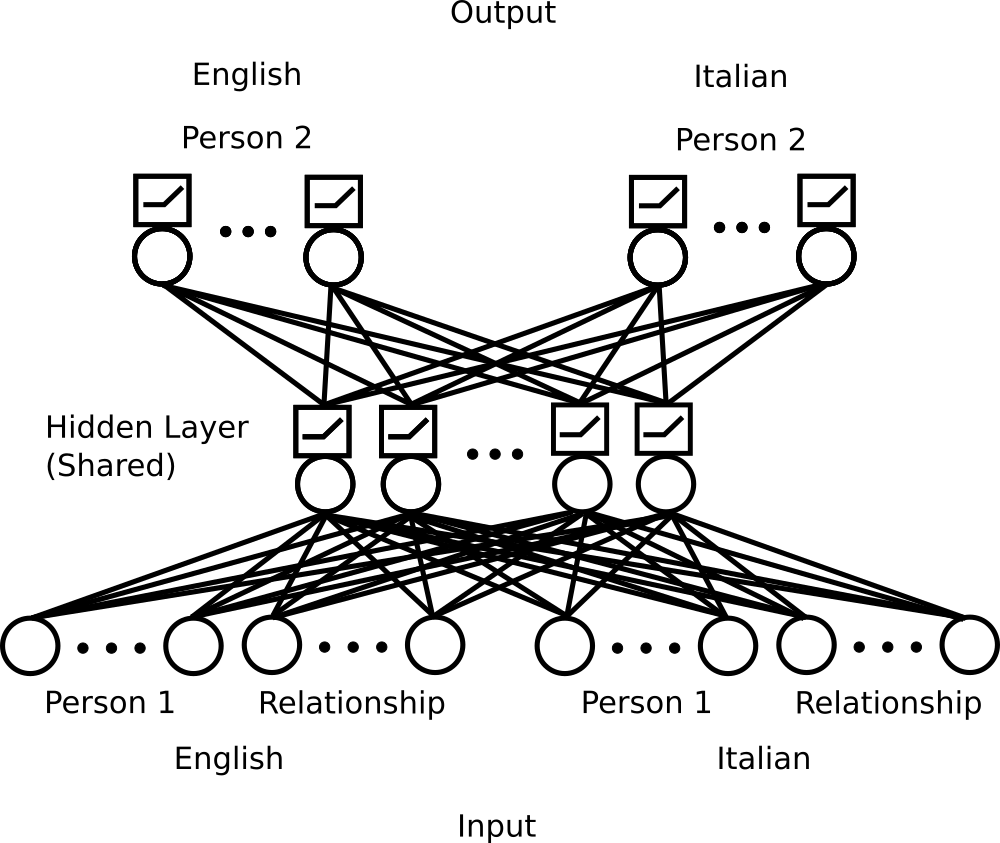
\includegraphics[width = \textwidth]{../writing/cogsci_2017/figures/family_tree_network_diagram.png}
    \end{center}
\end{columns}
\begin{itemize}
\item<2-> Our network is simplified from Hinton's, and tasks are completely separated.
\end{itemize}
\end{frame}

\begin{frame}{Hinton family tree task: Problems}
A few problems:
\begin{itemize}
    \item<2-> Task is not linearly separable, so we have multiple non-linearities, so how to perform analysis?
    \begin{itemize}
	\item<3-> The simple approach we took is just to perform the linearized analysis at each layer. 
    \end{itemize}
    \item<4-> Multiple analogies exist between family trees (for example flip left to right and reverse genders) 
    \only<4> {
    \begin{center}
	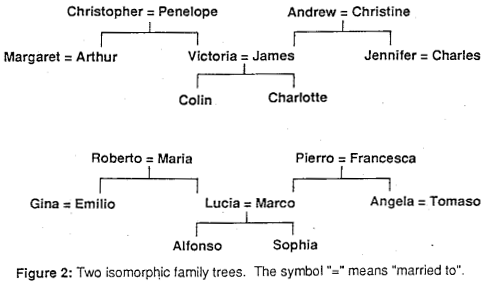
\includegraphics[width = 0.5\textwidth]{../writing/cogsci_2017/figures/hinton_family_tree_figure.png}
    \end{center}
    }
    \begin{itemize}
	\item<5-> Include both these analogies in our analysis. 
    \end{itemize}
    \item<6-> Cannot simply ``eyeball'' structure extraction here, need a principled measure of shared structure extraction. 
    \begin{itemize}
	\item<7-> Use a permutation test on each SVD mode to see whether the domains share more structure in this mode than would be expected by chance. 
    \end{itemize}
\end{itemize}
\note{Hinton shared relationship inputs, and had shared hidden layers, but we want to strip down to see if the analogies will emerge from the learning dynamics like in the above task.}
\end{frame}

\begin{frame}{Results}
Significant amounts of shared structure extraction!\\[11pt]
    \uncover<2->{
    First layer input modes:
    \begin{center}
    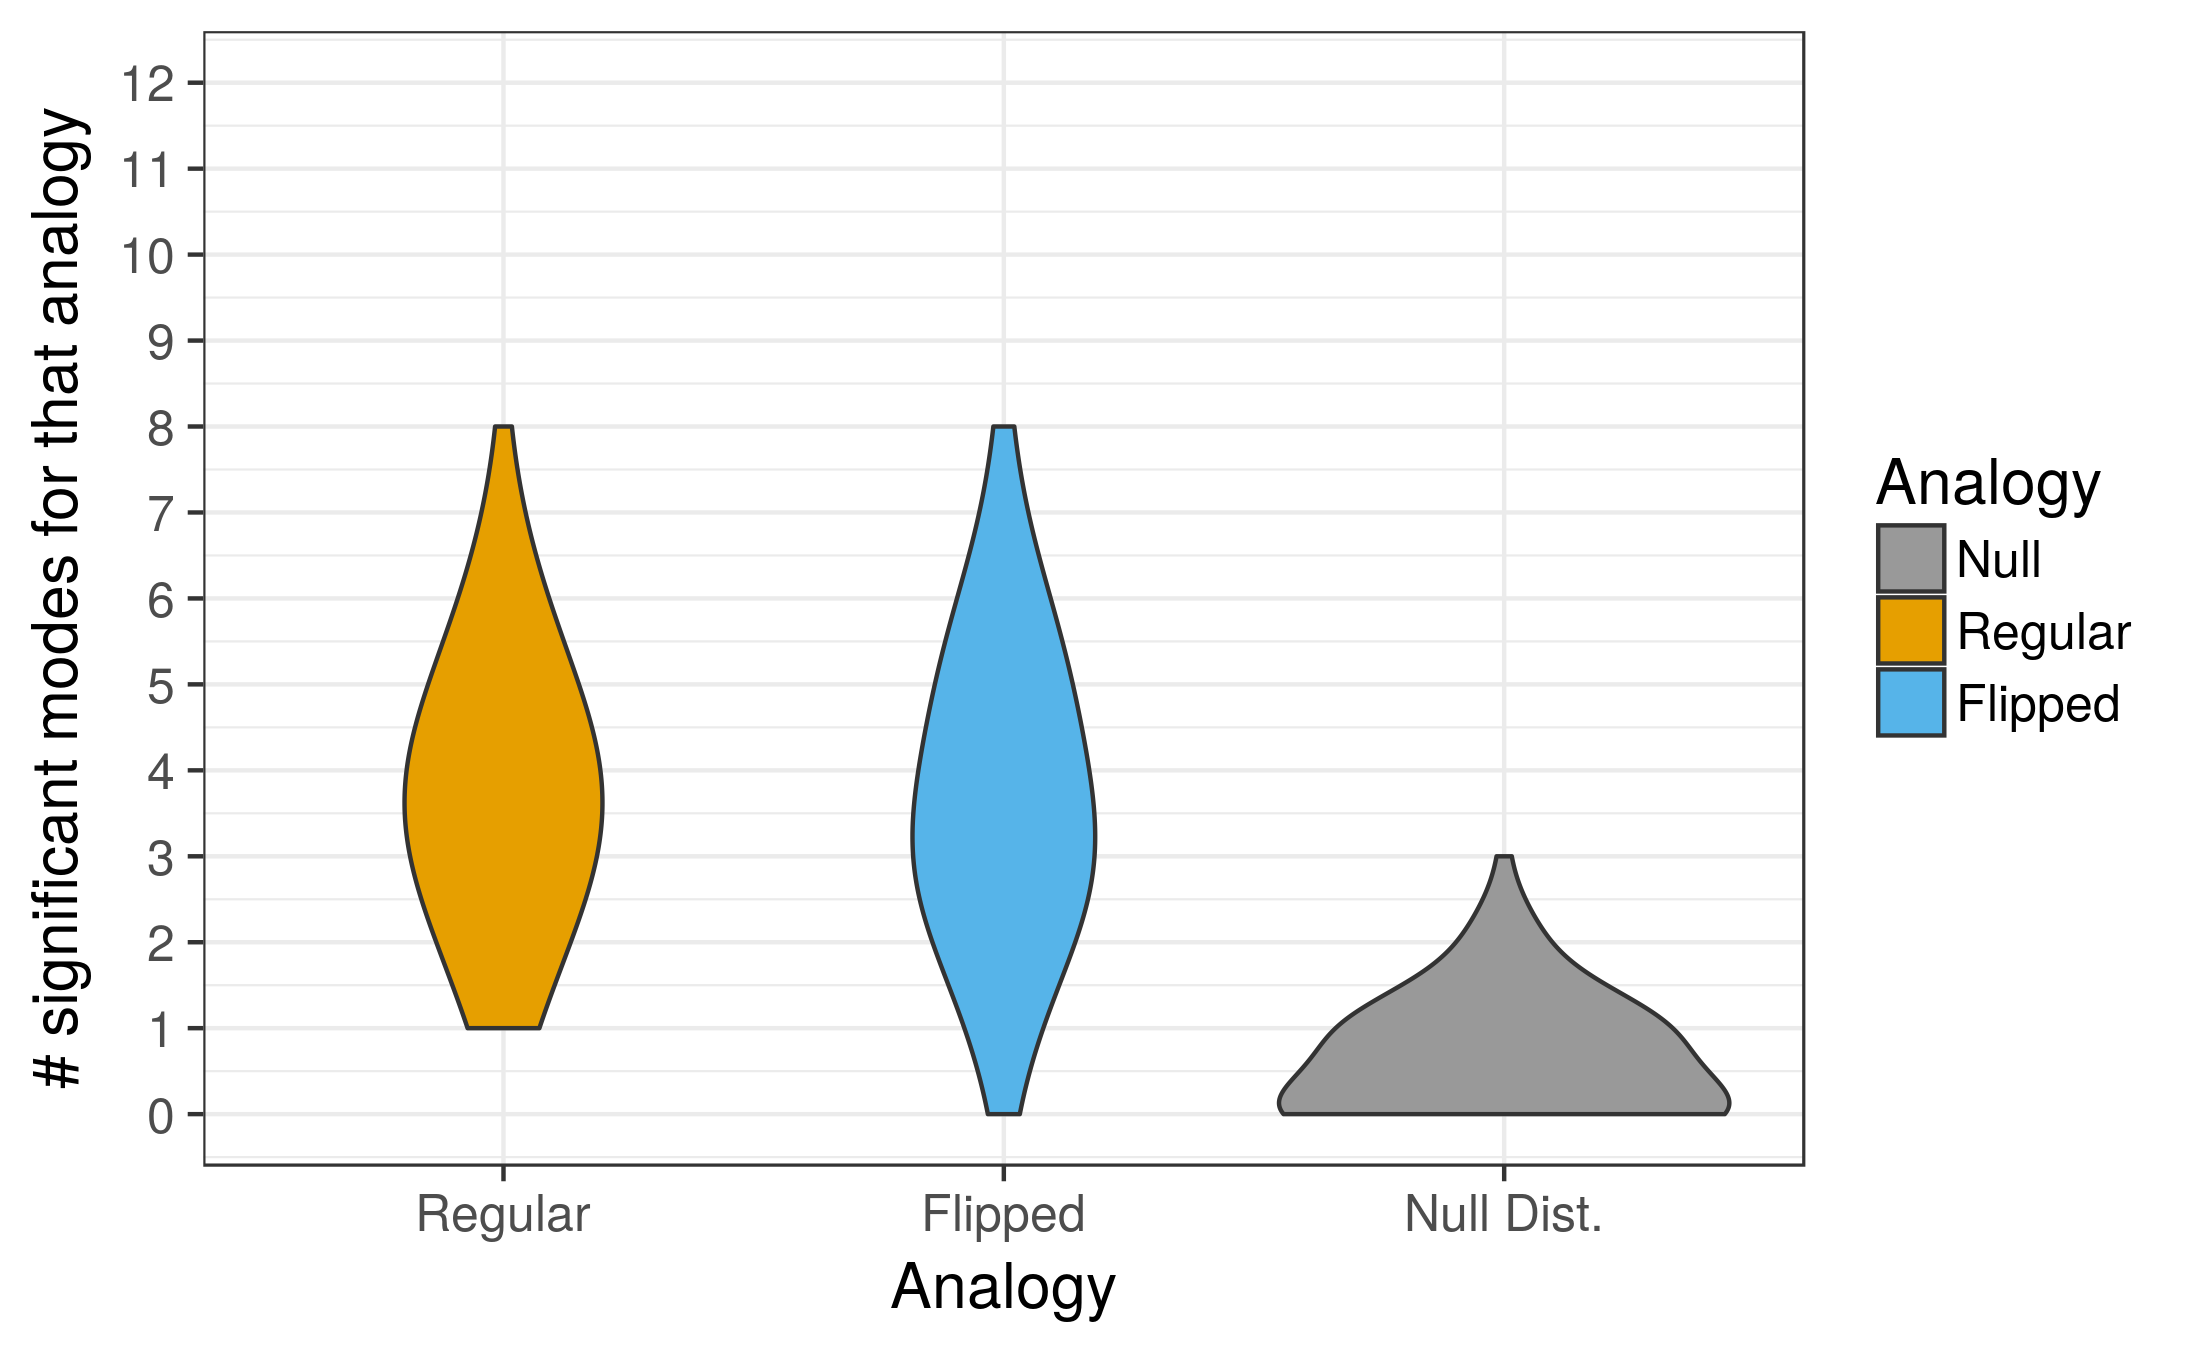
\includegraphics[width=0.75\textwidth]{../hinton_family_tree/results/input_mode_projections_violin.png} 
    \end{center}
    }
\end{frame}
\begin{frame}
Also in second layer output modes (although slightly less):
\begin{center}
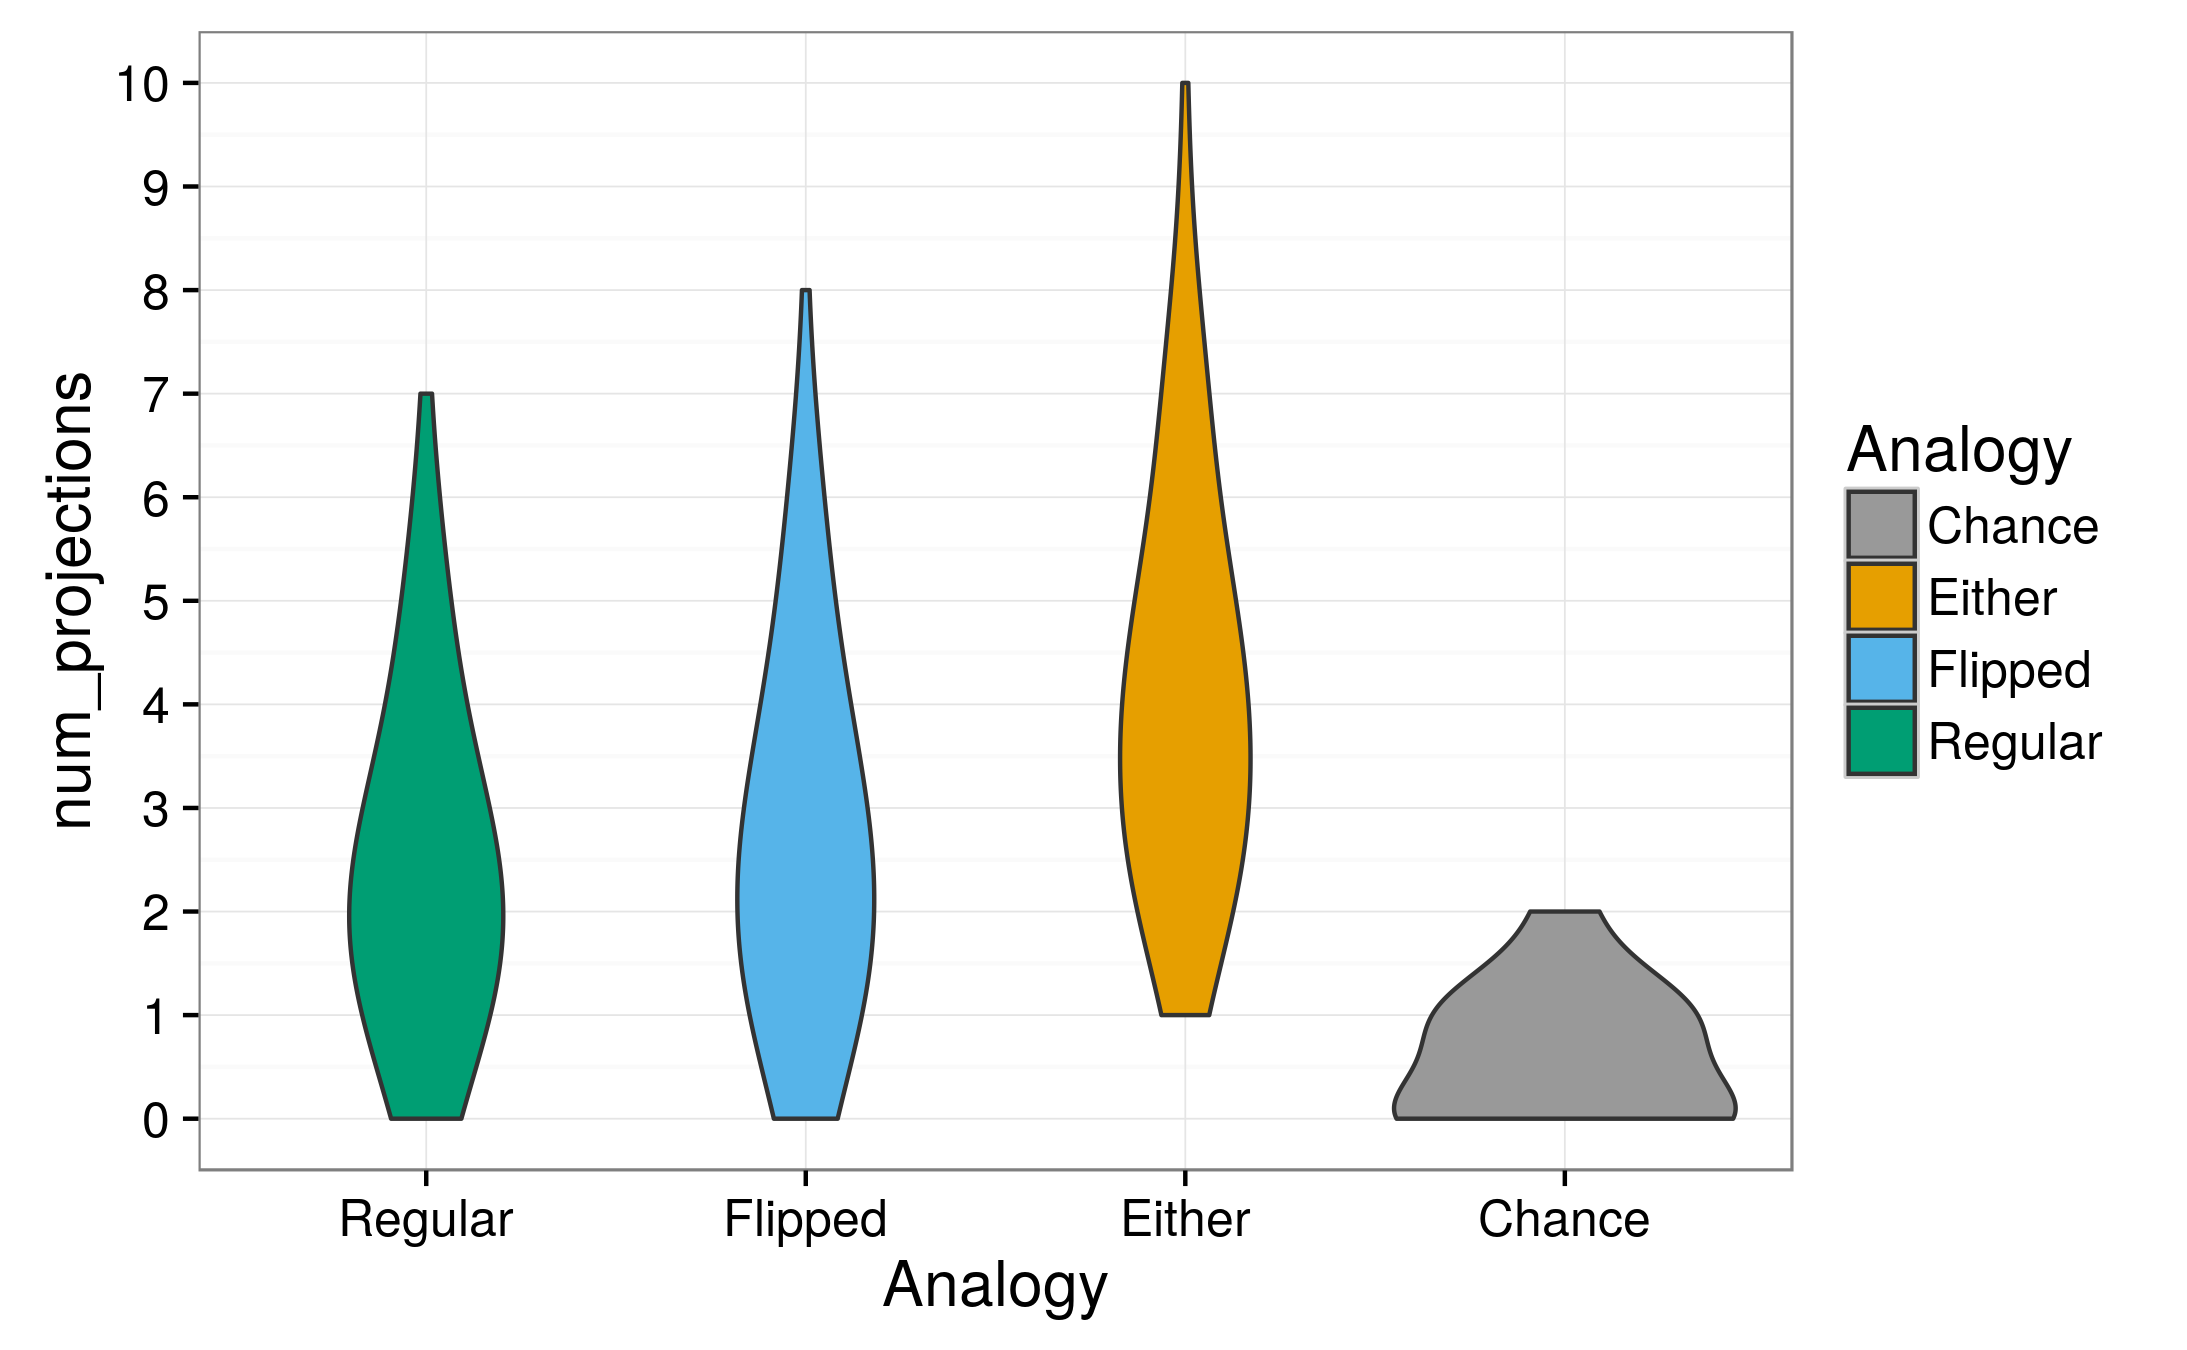
\includegraphics[width=0.75\textwidth]{../hinton_family_tree/results/output_mode_projections_violin.png} 
\end{center}
\end{frame}

\begin{frame}{Shared structure highlights:}
The input layers had:
\begin{itemize}
    \item<1-> A median of 6 modes showing significant extraction of the analogy to either the regular or flipped mapping (null: only 0.01\% of runs with 6 significant modes, median 0).
    \item<2-> 3 or more significant components from at one of the mappings alone in 95\% of the runs (null: in 4\% of runs).
    \item<3-> 3 or more significant components overall in all of the runs (null: in 3\% of runs).
\end{itemize}
\uncover<4->{Shared structure extraction appears \textbf{more consistent in a more complex task} than it was in the toy task}
\end{frame}

\begin{frame}{PFL Results}
Suppose we share some weights, can we see evidence of preparation for future learning?\\[11pt]
\begin{columns}
\column{0.45\textwidth}
    \uncover<2->{
    \begin{center}
    \includegraphics[width=\textwidth]{figures/shared_weights_network_diagram.png}
    \end{center}
    }
\column{0.45\textwidth}
    \uncover<3->{Yes, learning is faster after learning an analogous task than after learning a different one.
    \begin{center}
    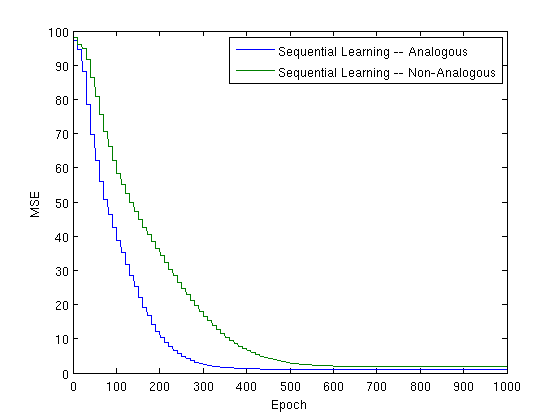
\includegraphics[width=1.1\textwidth]{figures/preparation_for_learning.png} 
    \end{center}
    }
\end{columns}
\note{Would expect this effect to increase with increasing depth of the network}
\end{frame}

\begin{frame}{PFL Results}
Does this still result in extraction of analogies? Yes, but not quite as much as learning simultaneously.\\[11pt]
\begin{columns}
\column{0.45\textwidth}
    \uncover<2->{
    Learn analogous task first:
    \begin{center}
    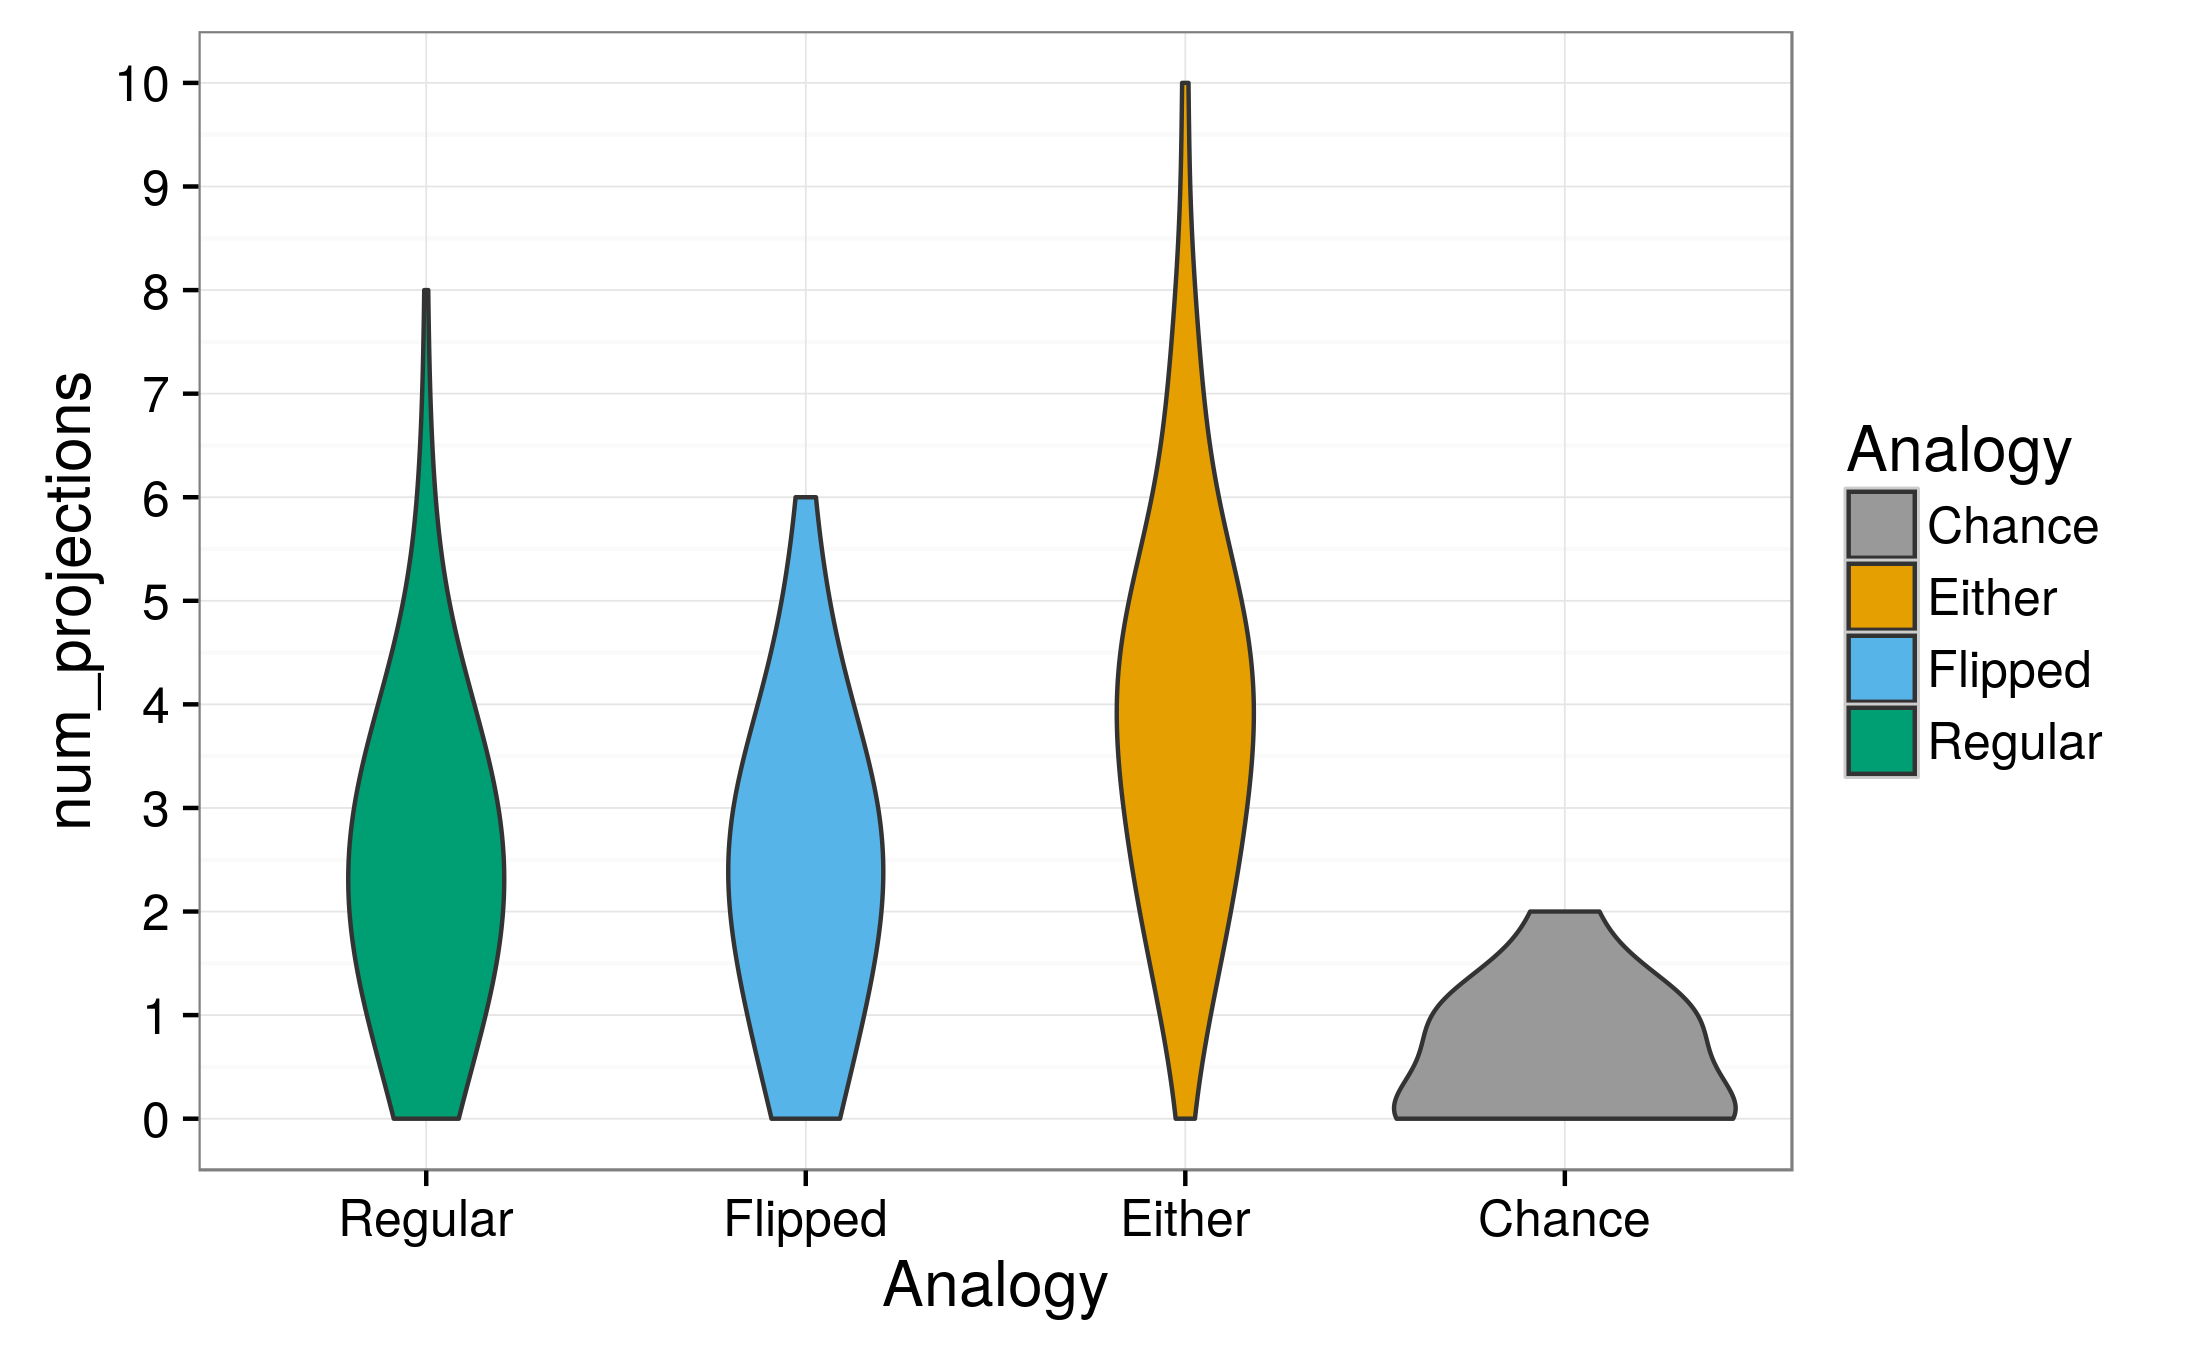
\includegraphics[width=1.2\textwidth]{../hinton_family_tree/results/pfl/anal_input_mode_projections_violin.png}
    \end{center}
    }
\column{0.45\textwidth}
    \uncover<3->{
    Learn different task first:
    \begin{center}
    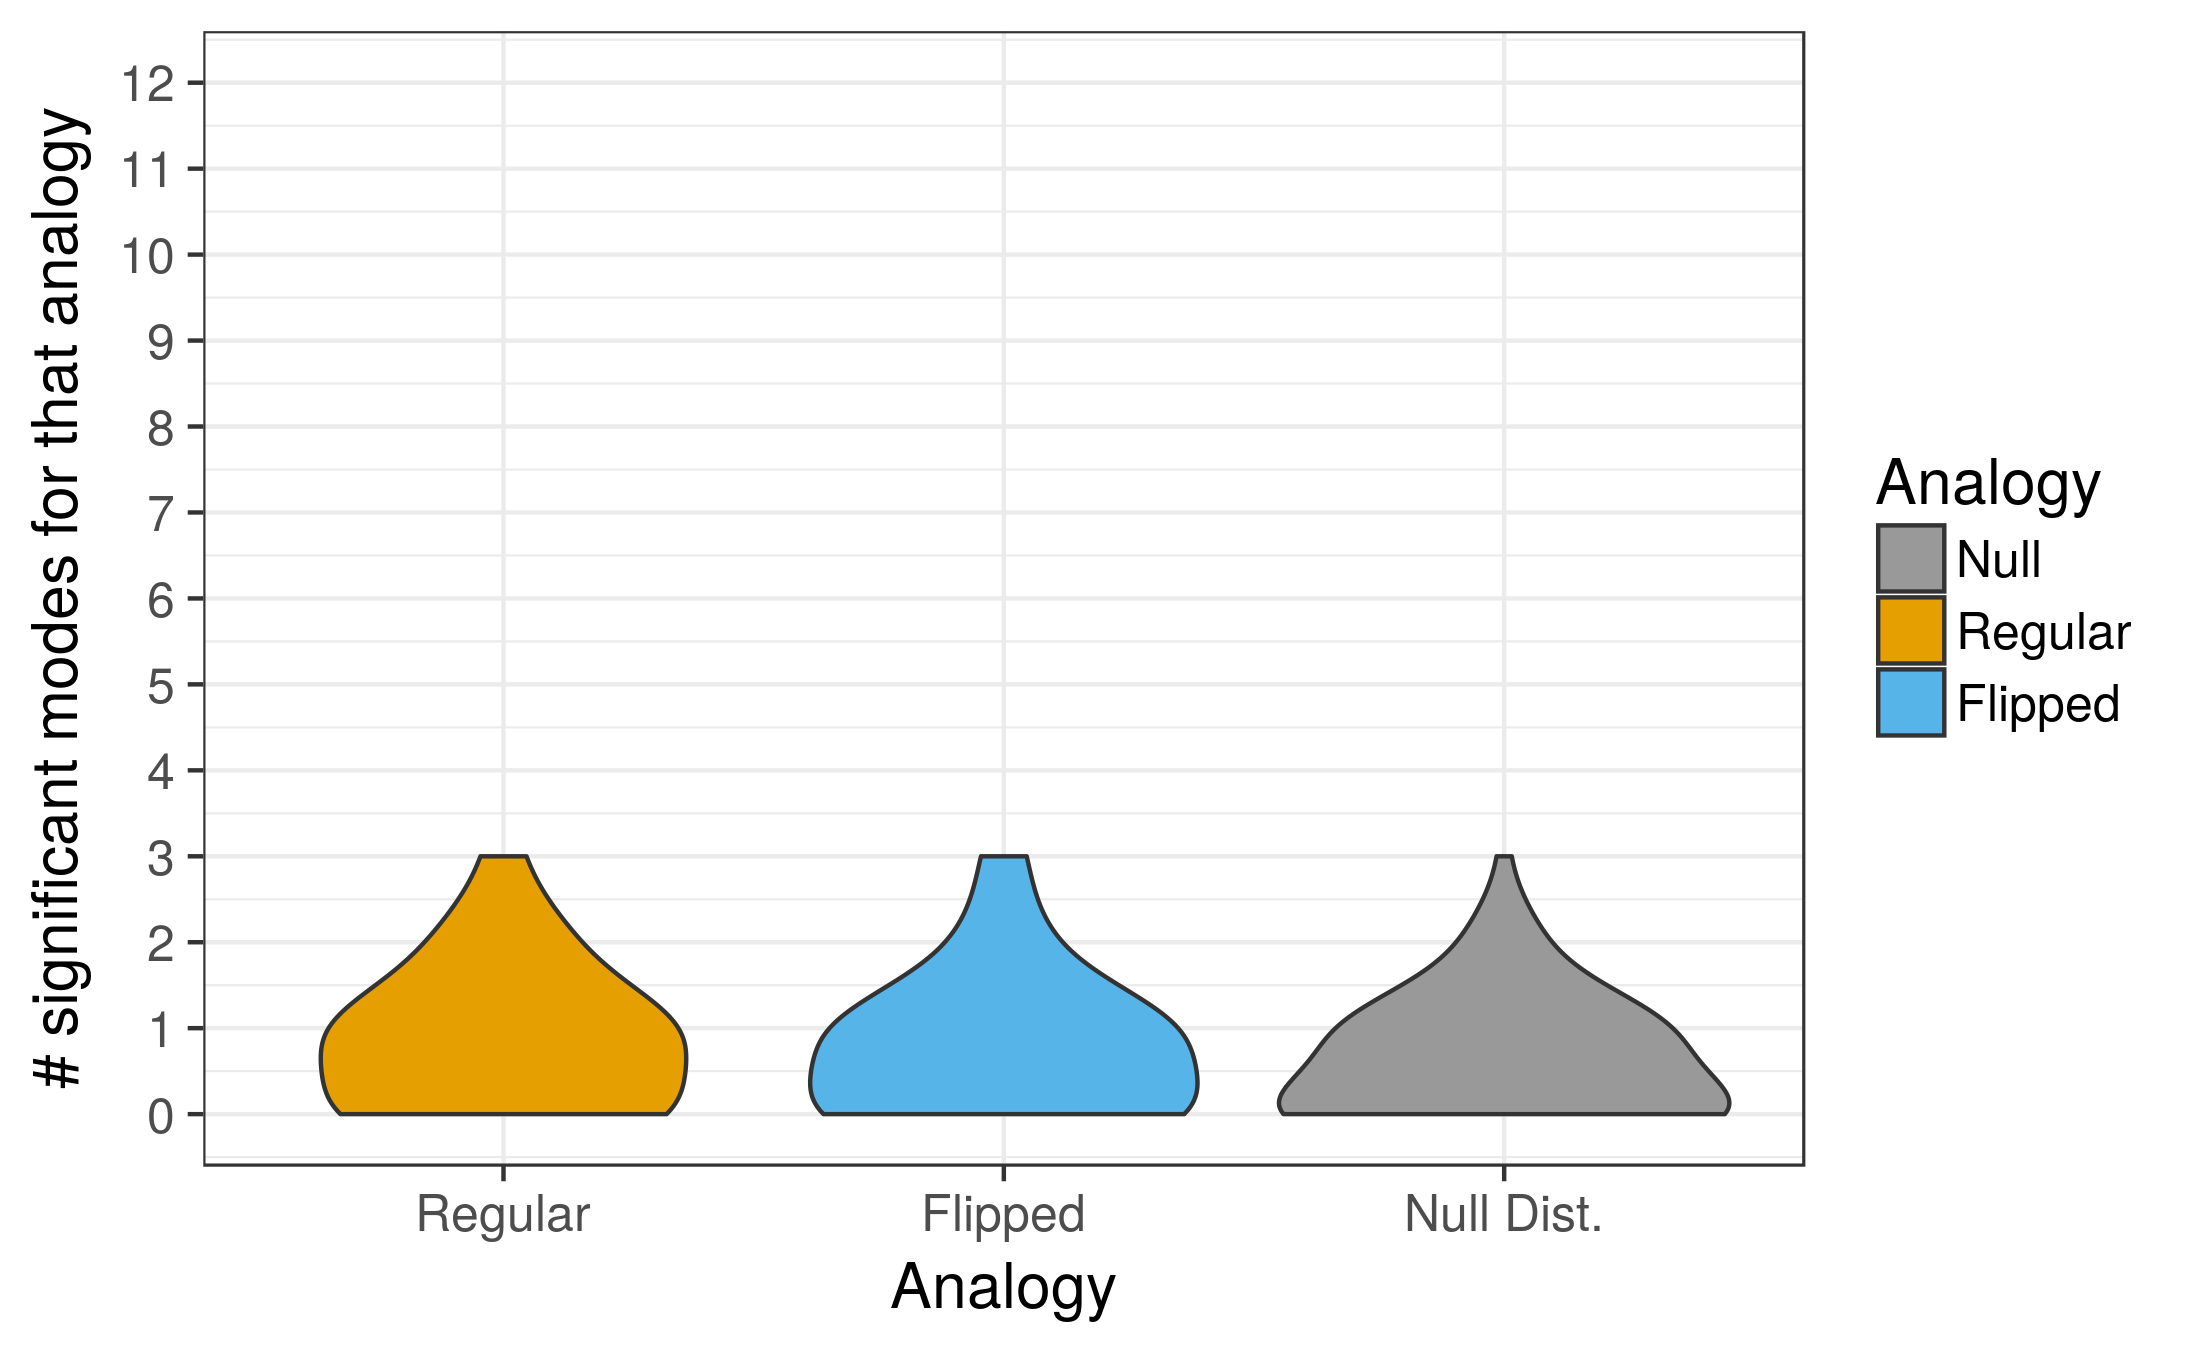
\includegraphics[width=1.2\textwidth]{../hinton_family_tree/results/pfl/alt_input_mode_projections_violin.png}
    \end{center}
    }
\end{columns}
\end{frame}

\section{Conclusions}

\begin{frame}{Results summary}
\begin{itemize}
    \item<1-> We outlined a new linearized analysis method for non-linear neural networks. 
    \item<2-> Used this in a toy task to show that analogies between non-overlapping tasks emerge naturally from learning dynamics. 
    \item<3-> Used in a more complicated task, and found that extraction of the analogies was even more consistent than on the toy task. 
    \item<4-> This extraction of analogies can emerge from:
    \begin{itemize}
	\item<5-> Simultaneous learning (or replay) without shared weights. 
	\item<6-> Non-simultaneous learning with shared weights.
    \end{itemize}
    \item<7-> This may provide a good model for ``slow'' human analogical reasoning and transfer, including:
    \begin{itemize}
	\item<8-> Possible amortized inference about analogies.
	\item<9-> Benefits of multiple mutually supporting tasks.
	\item<10-> Preparation for future learning.
    \end{itemize}
\end{itemize}
\end{frame}

\begin{frame}{Acknowledgements}
Thanks to:
\begin{itemize}
    \item Co-authors: Shaw Hsu \& Jay McClelland
    \item The rest of the lab for helpful conversations and feedback. 
    \item You, for listening.
\end{itemize}
\end{frame}

\begin{frame}[allowframebreaks]
\bibliographystyle{apacite}
\bibliography{shared_reps}
\end{frame}
\end{document}
